\subsubsection{Graph Viewer}
The Graph Viewer was implemented in the following manner:
\begin{description}
\item[HistoryGraph] This was used to hold and display an instance of the
ScatterChart class as well as load the Visualization API. It also
provides a communication interface between ScatterGraph and the rest of the
system. It also allows data to be added to or removed from the current chart.
\item[ScatterGraph] A container for a ScatterChart~\cite{scatter} which loads a new chart when provided with data.
\end{description}
\begin{figure}[h!]
\centering
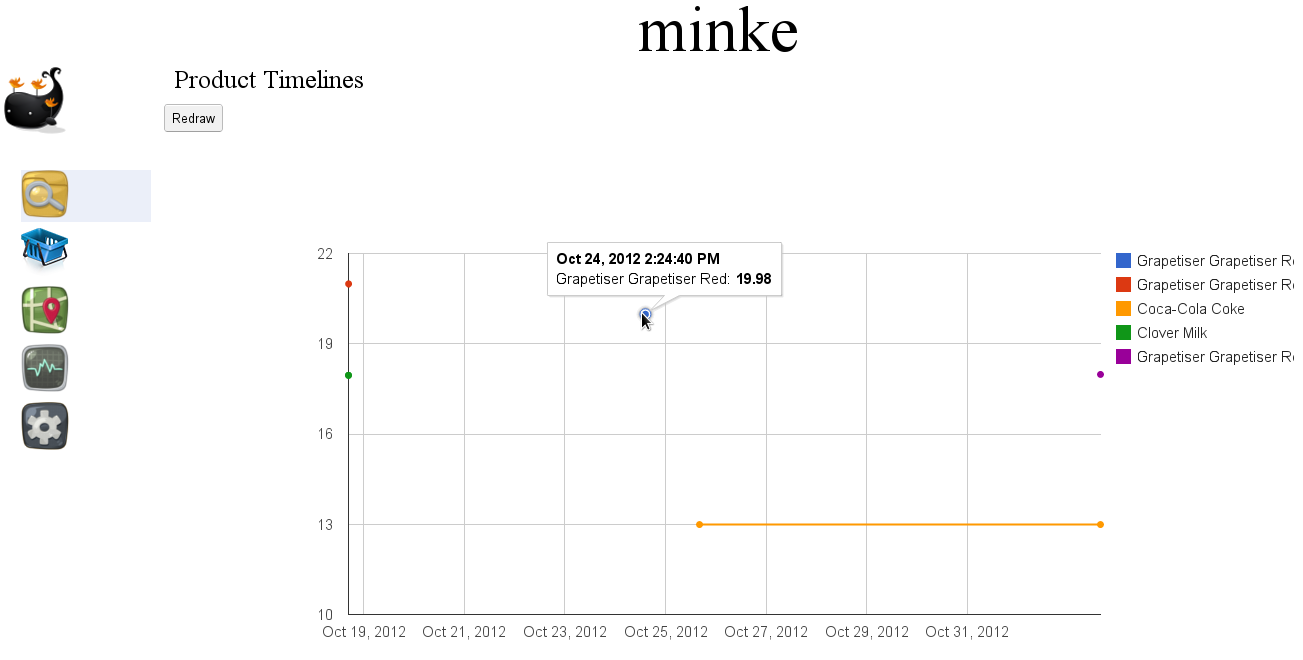
\includegraphics[width=1.0\textwidth]{gwt-graph.png}
\caption{The Graph Viewer interface.}
\end{figure}